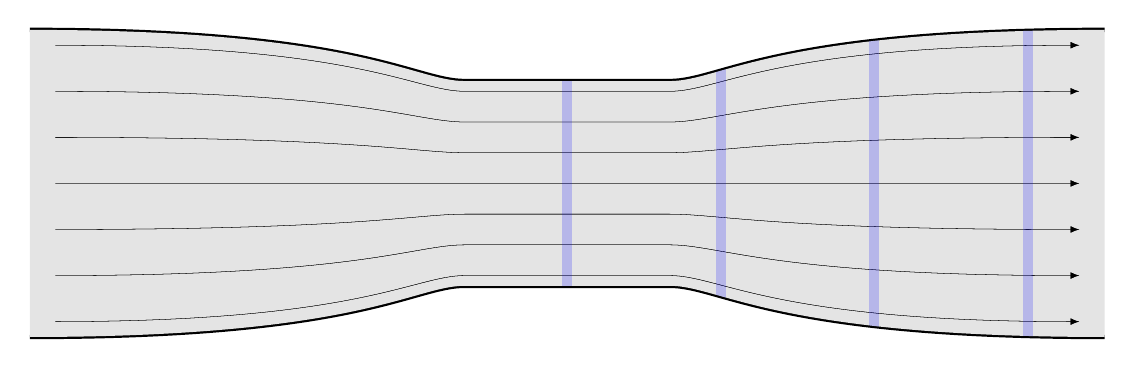
\begin{tikzpicture}[scale=0.65]
    \draw[ultra thick] (-10.5,+3) 
    .. controls(-4,+3) and (-3,+2) 
    .. (-2,+2)--(+2,+2) 
    .. controls (+3,+2) and (+4,+3) .. (+10.5,+3);

    \draw[ultra thick] (+10.5,-3) 
    .. controls(+4,-3) and (+3,-2) 
    .. (+2,-2)--(-2,-2) 
    .. controls (-3,-2) and (-4,-3) .. (-10.5,-3);

    \fill[black!10.5!white]
    (-10.5,+3) 
    .. controls(-4,+3) and (-3,+2) 
    .. (-2,+2)--(+2,+2) 
    .. controls (+3,+2) and (+4,+3) .. (+10.5,+3) -- 
    (+10.5,-3) 
    .. controls(+4,-3) and (+3,-2) 
    .. (+2,-2)--(-2,-2) 
    .. controls (-3,-2) and (-4,-3) .. (-10.5,-3) -- cycle;

    \foreach \x in {-0.9,-0.6,...,0.91}
    {
        \draw[ultra thin,-latex] (-10,+\fpeval{\x*3}) 
        .. controls(-4,+\fpeval{\x*3}) and (-3,+\fpeval{\x*2}) 
        .. (-2,+\fpeval{\x*2})--(+2,+\fpeval{\x*2}) 
        .. controls (+3,+\fpeval{\x*2}) and (+4,+\fpeval{\x*3}) .. (+10,+\fpeval{\x*3});
    
        \draw[ultra thin,-latex] (-10,-\fpeval{\x*3}) 
        .. controls(-4,-\fpeval{\x*3}) and (-3,-\fpeval{\x*2}) 
        .. (-2,-\fpeval{\x*2})--(+2,-\fpeval{\x*2}) 
        .. controls (+3,-\fpeval{\x*2}) and (+4,-\fpeval{\x*3}) .. (+10,-\fpeval{\x*3});
    }

    \clip
    (-10.5,+3) 
    .. controls(-4,+3) and (-3,+2) 
    .. (-2,+2)--(+2,+2) 
    .. controls (+3,+2) and (+4,+3) .. (+10.5,+3) -- 
    (+10.5,-3) 
    .. controls(+4,-3) and (+3,-2) 
    .. (+2,-2)--(-2,-2) 
    .. controls (-3,-2) and (-4,-3) .. (-10.5,-3) -- cycle;

    \fill[fill=blue,fill opacity=0.2] (-0.1,4) rectangle (0.1,-4);

    \fill[fill=blue,fill opacity=0.2] (2.9,4) rectangle (3.1,-4);

    \fill[fill=blue,fill opacity=0.2] (5.9,4) rectangle (6.1,-4);

    \fill[fill=blue,fill opacity=0.2] (8.9,4) rectangle (9.1,-4);
\end{tikzpicture}
